\documentclass[tikz,border=10pt]{standalone}
\usepackage{tikz}
\begin{document}
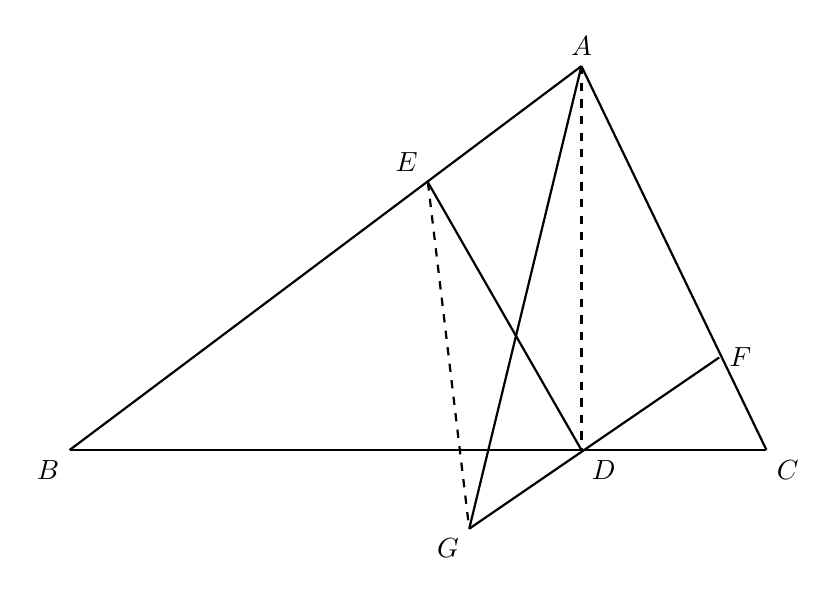
\begin{tikzpicture}[scale=1, line width=0.8pt]
  \coordinate (B) at (0,0);
  \coordinate (C) at (8.85,0);
  \coordinate (A) at (6.5,4.875);
  \coordinate (E) at (4.55,3.4);
  \coordinate (D) at (6.5,0);
  \coordinate (F) at (8.25,1.175);
  \coordinate (G) at (5.075,-1);

  \draw (B) -- (A);
  \draw (A) -- (C);
  \draw (B) -- (C);
  \draw (E) -- (D);
  \draw (A) -- (G);
  \draw (G) -- (F);
  \draw[dashed] (A) -- (D);
  \draw[dashed] (E) -- (G);

  \node[above left] at (E) {$E$};
  \node[above] at (A) {$A$};
  \node[below left] at (B) {$B$};
  \node[below right] at (C) {$C$};
  \node[below right] at (D) {$D$};
  \node[right] at (F) {$F$};
  \node[below left] at (G) {$G$};
\end{tikzpicture}
\end{document}
